\documentclass[12pt]{article}
\usepackage{graphicx} 		% Used to for importing images
\usepackage{indentfirst}	% Indents 1st paragraph (by default its off)
\usepackage{longtable} 		% Tables than can span over multiple pages
\usepackage{placeins}		% Used to keep images in place(via \FloatBarriers), and let text go infront
\usepackage[table]{xcolor}	% Used to colour specific table rows
\usepackage[hidelinks]{hyperref}		% Used to add hyperlinks
\usepackage[nottoc,numbib]{tocbibind}	% Used to include reference in Table of contents

% Define Global Variables
\setlength{\parindent}{20pt}
\graphicspath{ {/Diagrams} }

\begin{document}

\begin{titlepage}

% Defines a new command to draw horizontal lines
\newcommand{\Line}{\rule{\linewidth}{0.5mm}} 

% Center everything on the page
\center
 
% textsc - capitalizes every letter
\textsc{\LARGE University of Gothenburg}
% Define gap after text line
\\[3.5cm] 

% Course code and name
\textsc{\Large DIT168}\\[0.3cm]
\textsc{\large Project: Industrial IT and Embedded Systems}\\[0.5cm]

% Use the defined command to draw lines
\Line \\[0.4cm]
{\huge \bfseries Software Architectural Document}\\[0.4cm]
\Line \\[0.5cm]
 
% Large italic text
\Large \textit{Authors:}
\\Erik Laurin
\\Isabelle Törnqvist
\\Joacim Eberlen
\\Justinas Stirbys \\[4cm]

% Original date for the vision
{\large Group 01} \\[0.3cm]
{\large March 30th, 2018}

% Fills the remaining page with whitespace
\vfill

\end{titlepage}

% Creating table of contents
\tableofcontents
\pagebreak

% a SAD start
%%%%%%%%%%%%%%%%%%%%%%%%%%%%%%%%%%
% Add SAD history of changes table
%%%%%%%%%%%%%%%%%%%%%%%%%%%%%%%%%%

\section{Revision History} \label{sec:history}
The evolution of the Software Architectural Document for project dashFTABs is detailed under this section. Emphasis is put on changes incorporated, via Description column, the date and the author. In situation where all members have contributed to a change the author will be listed as Group 01.
% Define 4 aligned columns; l = left, c = center, r = right, the | = means vertical line    % \hline -> Draw horizontal line
% p{xcm} -> specifies how much space the column should take up, 
% 0.x\linewidth is used to make it p{} command more dynamic
\begin{longtable}{ | p{0.25\linewidth} | p{0.1\linewidth} | p{0.5\linewidth} | p{0.15\linewidth} | }\hline 
    \textbf{Date} & \textbf{Version} & \textbf{Description} & \textbf{Author} \\ \hline
   	27th March, 2018 & 0.1 & Added Functional Requirements & Group 01\\ \hline
   	4th April, 2018 & 0.2 & Added Introduction & Justinas\\ \hline
   	5th April, 2018 & 0.3 & Added Use Case View & Justinas\\ \hline
   	12th April, 2018 & 0.4 & Added Sequence Diagrams for UC1-UC3 & Justinas\\ \hline
	18th April, 2018 & 0.4.3 & Added 4+1 Vew Model to Introduction, UC1-UC3 sequence diagram descriptions to Process View & Justinas\\ \hline
	21st April, 2018 & 0.5 & Added System Context & Erik\\ \hline
    
    \rowcolor{blue!80!red!30} % Colour the row below in purple
	17th May, 2018 & 0.6 & Added Logical View (from "Conceptual Ideas") & Isabelle\\ \hline
    20th May, 2018 & 0.7 & Added Final Report subsection in Introduction, Drive Car Use Cases (UC), UC Significance and Behaviour subsections for Connect as Leader and Stop Following, and references for external libs & Justinas\\ \hline 
    
    \rowcolor{blue!80!red!30} % Colour the row below in purple
    20th May, 2018 & 0.8 & Added Physical View (from "Hardware \& Software Integration)& Justinas\\ \hline 
    
    \rowcolor{blue!80!red!30} % Colour the row below in purple
    20th May, 2018 & 0.9 & Added Maneuvering subsection to Process View (from "Algorithmic Fundamentals") & Erik\\  \hline
    
    \rowcolor{blue!80!red!30} % Colour the row below in purple
    20th May, 2018 & 1.0 & Added Development View (originally "Software Architecture" section) & Joacim\\ \hline
\end{longtable}

The rows coloured purple indicated parts of the document that were taken from the Final Report\cite{FinalReport}. Specific section of the Report are written in parenthesis. The only section to be taken fully from the Final Report is the Development View.
\pagebreak

%%%%%%%%%%%%%%%%%%%%%%%%%%%%%%
% Adding document introduction
%%%%%%%%%%%%%%%%%%%%%%%%%%%%%%
\section{Introduction}
\subsection{Purpose}
The purpose of this document is to familiarize the reader with the architectural overview of the software, developed for the project dashFTABs, by examining different architectural viewpoints. In continuation, the document includes architectural drivers, such as system requirements, and attempts to identify significant dashFTABs system’s behaviour.\par

%%%%%%%%%%%%%%%%%%%%%%%%%%%%%%
%%% New Subsection
\subsection{Scope}
The software was developed as part of the DIT168 Project: Industrial IT and Embedded Systems course taught at University of Gothenburg in Gothenburg, Sweden. The project course provides a 3D printed miniature car, dubbed Dash by the project group. The project groups communicate amongst each other to implement a Vehicle-to-Vehicle (V2V) protocol. Moreover, via incorporation of the protocol the project groups must expand Dash’s functional capabilities by implement platooning.\par

%%%%%%%%%%%%%%%%%%%%%%%%%%%%%%
%%% New Subsection
\subsection{Audience}
The document contains technical details of the project and utilizes Unified Modeling Language (UML for short) to express architecture. Therefore, the reader must possess some minimal or introductory knowledge of UML. As such the intended readers are members or somewhat affiliated with software engineering.

%%%%%%%%%%%%%%%%%%%%%%%%%%%%%%
%%% New Subsection    
\subsection{4+1 View Model}
To further narrow down the intended audience the document incorporates 4+1 View Model. The document will focus on architectural logical, process, development and physical views. With each view providing value to specific set of stakeholders. Logical View provides most benefit to the system's end-users as it addresses whether all desired functionality has been implemented; the Process View focuses on the overall system by depicting the subsystems, meaning microservices, interactions; Development View is aimed at developers as it focuses more on individual module contents; lastly, Physical View shows the physical distribution of software, thus it provides most value to system engineers. \par
The "+1" of the the 4+1 View Model refers to Scenarios, which are used to describe the system behaviour. The Scenarios provide value to all stakeholders as it attempts to encapsulate the system requirements. The Scenarios have been expressed as a Use Case View. \par

\subsection{Final Report Overlap}
The document has some overlap with the Final Report\cite{FinalReport}(by the same Group), as shown by the Revision History, Section \ref{sec:history}. The specified overlaps were initially written for the Final Report. However, these overlaps were of interest to the Software Architectural Document. Moreover, the overlapping sections were planned to be included in the SAD before the Final Report had been written. This can be seen by the previous "4+1 View Model" subsection.

\pagebreak

%%%%%%%%%%%%%%%%%%%%%%%%%%%%%%%%%%%%%%%%%%%%%%%%%%%
% Adding System Context section
%%%%%%%%%%%%%%%%%%%%%%%%%%%%%%%%%%%%%%%%%%%%%%%%%%%
\section{System Context}   
\subsection{Project Context}
Putting our software on the miniature car provides the user of the car with two main features; the ability to maneuver the car and the ability to make the car follow another car of the same type. The user controls, and maneuvers, the car through a web-based interface, the web remote controller, where one also can engage the car's following mode which shall result in the car starting to follow another.

A simple domain model was created further improve the understanding of data flow and the interactions between different system parts. 
%Adding image
\FloatBarrier % -> Wrap image with this, to make sure text does not go infront of image if theres room
\begin{figure}[ht!]
\centering
%Make image as wide as the line
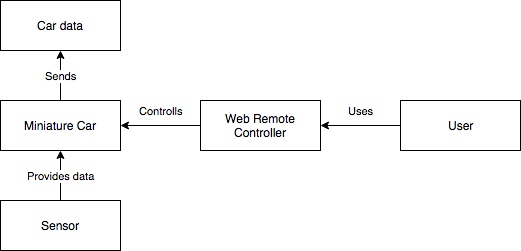
\includegraphics[width=\linewidth]{Diagrams/DomainModel.png}
\caption{Domain Model}
\label{fig:domainmodel}
\end{figure}
\FloatBarrier % -> Wrap image with this, to make sure text does not go infront of image if theres room

%%%%%%%%%%%%%%%%%%%%%%%%%%%%%%
%%% New Subsection    
\subsection{System Interface}
The software provides the user two way of interfacing with the car; the so called terminal remote controller and the web remote controller. 

The terminal remote controller provides the user with the ability to control the car through a simple computer terminal. Here, the user controls the car through the use of the keys. Furthermore, the user may also set the speed and the steering angle car should have when driving. Lastly, in case an obstacle is detected within a set distance, the car will break.

The more extensive web remote controller provides aforementioned features, (apart from being able to set the steering angle and distance before breaking for obstacles) together with another set of functionalities. Through the web remote controller, the car's speed, heading, distance traveled and the distance to obstacles are presented. In addition, most data that the car sends, receives and processes are displayed in the interface. Lastly, the interface provides the user with a switch that chooses which mode the car shall be in; leader (the user controls the car) or follower (the car follows another car autonomously).

%%%%%%%%%%%%%%%%%%%%%%%%%%%%%%
%%% New Subsection    
\subsection{External Libraries/Images}
To realize our software, various libraries and Docker images were used.

\begin{longtable}{ | p{0.15\linewidth} | p{0.85\linewidth} | }\hline 
	\textbf{Name} & \textbf{Description} \\ \hline
	libcluon\cite{libcluon} & Christian Berger's C++ library libcluon is the hub of our software. It is used for all communication, both internally in the car and externally to other car's.\\ \hline
    seresearch/ 2018-dit-168 & From this image we run two microservices, odsupercomponent and the proxy-miniature-pwm-motor which allow our software to control the miniature car through sending messages with the libcluon library.\\ \hline
	opendlv-device-ultrasonic-srf08-armhf & This image gets the front ultrasonic sensor's reading and make it available for our code to use.\\ \hline
    Robotics Cape\cite{robotics cape} & This library allows our software to access data readings from the sensors that are placed on the BeagleBone.\\ \hline
    opendlv-signal-viewer\cite{signal viewer} & This library was used as the base of the built web interface\\ \hline
\end{longtable}

\pagebreak


%%%%%%%%%%%%%%%%%%%%%%%%%%%%%%%%%%%%%%%%%%%%%%%%%%%
% Adding section detailing architecture motivations
%%%%%%%%%%%%%%%%%%%%%%%%%%%%%%%%%%%%%%%%%%%%%%%%%%%
\section{Architectural Drivers}
\subsection{Functional Requirements}
Functional requirements were used to identify and narrow down the project scope. The requirements are prioritized using MoSCoW notation i.e. requirements are divided into Must, Shoulds, Coulds, and Wont’s. Must dictates requirements that are mandatory for the final demonstration. Should expresses requirements that are significant, but do not have a defined deadline. Could expresses requirements/features that would improve the project quality, but are not necessarily implemented. Lastly, Won’t is used to track identified requirements that will not be implemented, due to product owner dislike or disapproval, time and budgetary constraints.\par

% Functional requirement table
% Define 4 aligned columns; l = left, c = center, r = right, the | = means vertical line    % \hline -> Draw horizontal line
\begin{longtable}{| p{0.05\linewidth} | p{0.15\linewidth} | p{0.45\linewidth} | p{0.25\linewidth} | p{0.1\linewidth} |}\hline 
    ID & Requirement & Description & Status & Priority \\ \hline
   	F1 & Message Log & A web page must contain a message log of everything that has been sent internally and externally within the car & Implemented & Must\\ \hline
   	F2 & Remote Controller & A web page must contain a graphical remote controller that communicates and controls Dash, when the car is the leader of the platoon & Implemented & Must\\ \hline
   	F4 & Leader Connection & The car, Dash, must be able to support Leader functionality (i.e. send LeaderStatus requests) while platooning & Implemented & Must\\ \hline       
    F5 & Follower Connection & The car, Dash, must be able to participate in platooning as a follower & Implemented & Must\\ \hline
    F6 & Maneuvering & The car will drive forward, turn left or right on commands received over the OD4 session & Implemented & Must\\ \hline
   	F7 & IMU & Dash must be able to use the IMU on its BeagleBoard Blue to calculate the distance moved & Implemented & Must\\ \hline
   	F8 & V2V Protocol & The car must be able to support the V2V Protocol. It is required for it to communicate with other cars and send sensors data & Implemented & Must\\ \hline
   	F9 & Collision Prevention & Dash will stop/brake when ultrasonic readings return an object that is less or equals to 10 cm ahead &  Implemented & Should\\ \hline
   	F10 & Emergency Brake & The car will stop if it fails to receive 3 update requests (i.e. hasn’t received anything in 300ms) and/or the connection to other cars has been lost & Implemented & Must\\ \hline
    F11 & Video Streaming& The car could incorporate the RPi and camera to live stream it’s video & Not Implemented & Could\\ \hline
  	F12 & Lane Following & Via incorporation of the RPi camera, Dash could implement identification and following of straight lines & Not Implemented & Could\\ \hline
\end{longtable}
\pagebreak


%%%%%%%%%%%%%%%%%%%%%%%%%%%%%%%%%%%%%%%%
% Adding section about project use cases
%%%%%%%%%%%%%%%%%%%%%%%%%%%%%%%%%%%%%%%%
\section{Use Case View}
This document section attempts to identify the main behaviour exhibited by Dash. This is done by expressing the behaviour as use case scenarios. The chosen scenarios depicts some of the significant features of developed project. Moreover, the identified scenarios all utilize the V2V Protocol in different aspects, meaning the use case scenarios use different messages from the protocol. Therefore, the identified scenarios fulfil different aspects of the functional requirements of F8 (V2V Protocol). \par

\subsection{Use Case Scenarios}

%%%%%%%%%%%%%%%%%%%%%%%%%%%%%%
%%% Use Case 1 Table
\subsubsection{Connect As Follower} \label{us:connect follower}
\begin{longtable}{| p{0.2\linewidth} | p{0.8\linewidth} |}\hline 
    ID & UC1\\ \hline
    Use Case & Connect as Follower\\ \hline
    Description & Dash connects to another miniature car as a Follower and begins to receiving Leader Status update messages\\ \hline
    Actors & Dash, Another Car\\ \hline
    Preconditions & Excluding Dash there is another miniature car with the V2V protocol that are not already connected to any cars\\ \hline
    Steps & Basic Flow: \begin{enumerate} % enumerate creates a numbered list
    	\itemsep 0em % -> Specify gaps between numbers in list 
    	\item Dash uses Announce Presence (it’s not very effective). Another car receives Dash’s IP and group number
		\item Another Car announces presence. Dash receives it’s IP and group number
        \item Dash uses Follow Requests. Selects which group car to follow
        \item Another Car receives follow request and does not have a follower yet. Another Car sends Follow Response
        \item A connection using UDP Sender and Receiver is established between Dash and Another Car 
        \end{enumerate}
        Alternative Flow: \begin{enumerate}
        	\setcounter{enumi}{3} % -> Starts list from a different specified index + 1
        	\item Another Car already has a Follower. 
            \begin{enumerate} % -> nested enumerates, index list. Default index 1->a->i->A
            	\itemsep 0em % -> Specify gaps between numbers in list 
         		\item No Follower Request is sent
         		\item Display a message informing the users
               	\item Continues at Basic Flow 2
       		\end{enumerate}
       	\end{enumerate}\\ \hline
\end{longtable}

%%%%%%%%%%%%%%%%%%%%%%%%%%%%%%
%%% Use Case 2 Table
\subsubsection{Connect As Leader}\label{us:conenct leader}
\begin{longtable}{| p{0.2\linewidth} | p{0.8\linewidth} |}\hline 
    ID & UC2\\ \hline
    Use Case & Connect as Leader\\ \hline
    Description & Dash connects to another miniature car as a Leader and begins to sending Leader Status update messages\\ \hline
    Actors & Dash, Another Car\\ \hline
    Preconditions & Excluding Dash there is another miniature car with the V2V protocol that are not already connected to any cars\\ \hline
    Steps & Basic Flow: \begin{enumerate} % enumerate creates a numbered list
        \itemsep 0em % -> Specify gaps between numbers in list 
    	\item Dash uses Announce Presence (it’s not very effective). Another car receives Dash’s IP and group number
		\item Another Car announces presence. Dash receives it’s IP and group number
        \item Dash receives follow request and does not have a follower yet. Dash sends Follow Response
        \item Another Car receives follow request and does not have a follower yet. Another Car sends Follow Response
        \item A connection using UDP Sender and Receiver is established between Dash and Another Car 
        \end{enumerate}
        Alternative Flow: \begin{enumerate}
        	\setcounter{enumi}{3} % -> Starts list from a different specified index + 1
        	\item Dash already has a Follower. 
            \begin{enumerate} % -> nested enumerates, index list. Default index 1->a->i->A
            	\itemsep 0em % -> Specify gaps between numbers in list 
         		\item No Follower Request is sent
         		\item Display a message informing the users
               	\item Continues at Basic Flow 2
       		\end{enumerate}
       	\end{enumerate}\\ \hline
\end{longtable}

%%%%%%%%%%%%%%%%%%%%%%%%%%%%%%
%%% Use Case 3 Table
\subsubsection{Stop Following Leader}\label{us:stop follow}
\begin{longtable}{| p{0.2\linewidth} | p{0.8\linewidth} |}\hline 
    ID & UC3\\ \hline
    Use Case & Connect as Leader\\ \hline
    Description & Dash disconnect from Another Car, which acted as a Leader\\ \hline
    Actors & Dash, Another Car\\ \hline
    Preconditions & Dash is already connected as a Follower to Another Car\\ \hline
    Steps & Basic Flow: \begin{enumerate} % enumerate creates a numbered list
        \itemsep 0em % -> Specify gaps between numbers in list 
    	\item Dash sends Follower Status and receives Leader Status, indicating it’s following Another Car
		\item Dash sends Stop Following message and stops moving
        \item Dash removes Another Car as it’s leader
        \item Another Car receives stop following message. Another Car removes Dash as it’s follower
	\end{enumerate}\\ \hline
\end{longtable}

%%%%%%%%%%%%%%%%%%%%%%%%%%%%%%
%%% New Section
\subsubsection{Drive Dash}\label{us:drive car}
The Drive Dash is comprised of 2 Use Cases. The first one depicts the scenario when Dash is leading another vehicle, the latter when Dash is being lead by another miniature vehicle.
%%%%%%%%%%%%%%%%%%%%%%%%%%%%%%
%%% Use Case 4
\begin{longtable}{| p{0.2\linewidth} | p{0.8\linewidth} |}\hline 
    ID & UC4\\ \hline
    Use Case & Drive as Leader\\ \hline
    Description & Another Car connects to Dash as a Follower, at which point a Driver uses the remote controller to maneuver Dash\\ \hline
    Actors & Dash, Driver, Another Car\\ \hline
    Preconditions & Another Car is already connected to Dash as a Follower\\ \hline
    Steps & Basic Flow: \begin{enumerate} % enumerate creates a numbered list
        \itemsep 0em % -> Specify gaps between numbers in list 
    	\item The Driver enables "Leader Role" through web interface.
        \item Dash swaps to leader mode.
        \item The Driver uses "WASD" keys to control Dash. Dash moves.
        \item Dash sends LeaderStatus to Another Car
	\end{enumerate}
    Alternative Flow: \begin{enumerate}
        	\setcounter{enumi}{2} % -> Starts list from a different specified index + 1
        	\item Dash detects an object ahead 
            \begin{enumerate} % -> nested enumerates, index list. Default index 1->a->i->A
            	\itemsep 0em % -> Specify gaps between numbers in list 
         		\item Dash stops
       		\end{enumerate}
       	\end{enumerate}\\ \hline
\end{longtable}

%%%%%%%%%%%%%%%%%%%%%%%%%%%%%%
%%% Use Case 5
\begin{longtable}{| p{0.2\linewidth} | p{0.8\linewidth} |}\hline 
    ID & UC5\\ \hline
    Use Case & Drive as Follower \\ \hline
    Description & Dash connects as a Follower to Another Car and begins autonomous moving\\ \hline
    Actors & Dash, Driver, Another Car\\ \hline
    Preconditions & Dash is connected as Follower to Another Car\\ \hline
    Steps & Basic Flow: \begin{enumerate} % enumerate creates a numbered list
        \itemsep 0em % -> Specify gaps between numbers in list 
    	\item The Driver enables "Follower Role" through web interface.
        \item The "WASD" keys used for moving are disabled.
        \item Dash swaps to follower mode.
        \item Dash receives LeaderStatus from Another Car.
        \item Dash queues LeaderStatus and begins driving using "speed" from LeaderStatus.
        \item Maximum queue size is met. Dash begins turning with "steeringAngle" from LeaderStatus that were queue.
        \item Dash removes top item from queue.
	\end{enumerate}
    Alternative Flow: \begin{enumerate}
        	\setcounter{enumi}{4} % -> Starts list from a different specified index + 1
        	\item Dash is not in follower mode
            \begin{enumerate} % -> nested enumerates, index list. Default index 1->a->i->A
            	\itemsep 0em % -> Specify gaps between numbers in list 
         		\item Dash ignores messages
                \item Retry Basic Flow 2
       		\end{enumerate}
       	\end{enumerate}\\ \hline
\end{longtable}

%%%%%%%%%%%%%%%%%%%%%%%%%%%%%%
%%% New Subsection
\subsection{Use Case Diagram}
To depict use case interactions amongst each other, a use case diagram was created.

\FloatBarrier % -> Wrap image with this, to make sure text does not go infront of image if theres room
% Adding use case diagram image
\begin{figure}[ht!]
\centering
% Make image as wide as the line
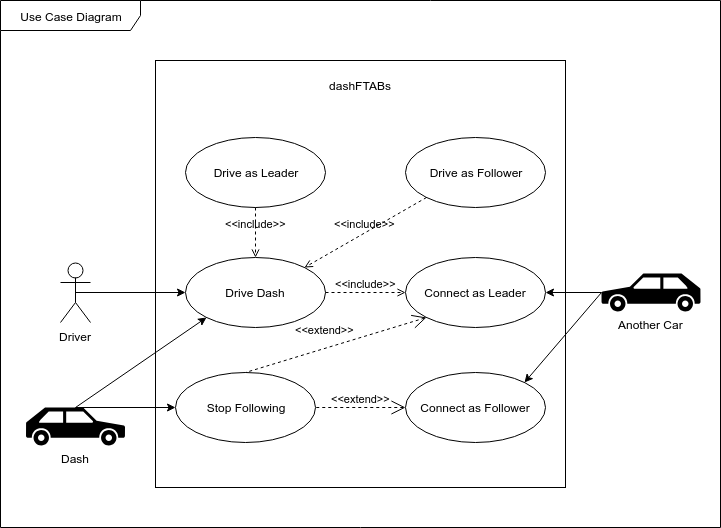
\includegraphics[width=\linewidth]{Diagrams/UseCaseDiagram.png}
\caption{Use Case Diagram}
\label{fig:usecasediagram}
\end{figure}
\FloatBarrier % -> Wrap image with this, to make sure text does not go infront of image if theres room
The diagram also servers as a visual aid, aimed to improve understanding of actor interactions with project functionality, as such it could also be included in the Logical View. However, it was believed its best served to tie in together all established Use Cases, as the diagram depicts the interactions between the most significant use case scenarios, mentioned in previous sections.
 
\pagebreak
%%%%%%%%%%%%%%%%%%%%%%%%%%%%%%%%%%%%%%%%%%%%%%%%%
% Adding section about microservice communication
%%%%%%%%%%%%%%%%%%%%%%%%%%%%%%%%%%%%%%%%%%%%%%%%%
\section{Process View}
The Process View section aims to inform the reader on subjects such as communication between the designed software components and communication between the project's subsystem i.e. the developed microservices. The section graphically express the architecturally significant use cases (See section Use Case View). Sequence Diagrams (SD for short) were used for use case realization, while natural language was used to improve the readers’ understanding of the architectural significance the use cases provide.\par

\subsection{V2V Protocol}
As the focus for the project is vehicle-to-vehicle (V2V) communication, a shared V2V protocol was developed by a representative from each team for the purpose of being utilized in the project. The project group dashFTABs has altered the provided protocol to accommodate their team's needs. The changes introduced do not go against any established agreements as the protocol is licensed under GNU General Public License v3.0, a license allowing modification. Moreover, the protocol was design in a way that would require small alterations to accommodative individual teams architecture. Due to the protocol being used by all project groups the behaviour exhibited by Connect as Leader, Connect as Follower will be similar across all teams.\par
The specific changes to the protocol include; creating an additional OD4 session for internal car communication, broadcasting the messages received from other cars to the internal channel, as well as an additional function responsible for monitoring time Leader/Follower Status request have been received. \par  

%%%%%%%%%%%%%%%%%%%%%%%%%%%%%%
%%% Connect As Follower
\subsection{Connect As Follower}
\subsubsection{Significance}
 The use case was chosen as architecturally significant, as it implements functional requirement F5, Follower Connection. The requirement itself was provided by the DIT168 course representatives, as it is mandatory for every miniature vehicle to posses follower capabilities. Without a follower connection, Dash would not be able to have automated moving or platooning, as it would not receive status updates from the leader. Therefore, F5 requirement acts as a prerequisite to more advanced functionality. Due to these reasons the requirement was deemed as significant and expressed as a sequence diagram. The sequence diagram depicts the behavior of UC1.\par

% Adding image
\FloatBarrier % -> Wrap image with this, to make sure text does not go in front of image if theres room
\begin{figure}[ht!]
\centering
% Make image as wide as the line
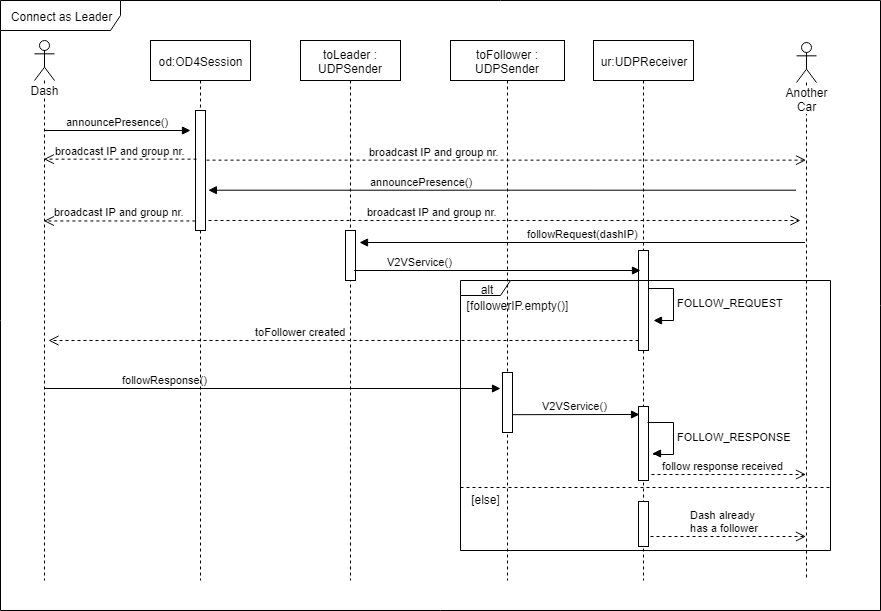
\includegraphics[width=\linewidth]{Diagrams/ConnectAsFollower.png}
\caption{Connect As Follower SD}
\label{fig:connectasfollower}
\end{figure}
\FloatBarrier % -> Wrap image with this, to make sure text does not go infront of image if theres room

\subsubsection{Behaviour} \label{subsubsec: follower bahaviour}
The interactions depicted in Figure \ref{fig:connectasfollower} focus specifically on behaviour exhibited by the V2V microservice. The diagram consists of 5 main components; OD4 Sessions broadcast and internal, UPD Senders toLeader, toFollower, and receiver a UDP Receiver. The broadcast OD4 session listens to CID 250, a channel used for cars that wish to engage in platooning. Once a car has used announcePresence() their car IP and group number are broadcasted to everyone on the network. Dash then send a FollowRequest, that is evaluated on the UDP Receiver. If Another Car does not have any followers it send a FollowResponce and uses Dasd's IP to establish a toFollower channel. Once Dash receives the FollowResponce message it creates a toLeader UDP Sender and the message exchange can begin. It is worth stating taht after every message is sent or received it is forwarder to "internal" OD4 session for data visualization.\par

%%%%%%%%%%%%%%%%%%%%%%%%%%%%%%
%%% Connect As Leader
\subsection{Connect As Leader}
\subsubsection{Significance}
Similarly to UC1, this use case was chosen for being a precursor to more advance behavior. To fulfil the project requirement the car must be able to create a connection as Leader and send LeaderStatus to realize V2V following.\par
% Adding image
\FloatBarrier % -> Wrap image with this, to make sure text does not go infront of image if theres room
\begin{figure}[ht!]
\centering
% Make image as wide as the line
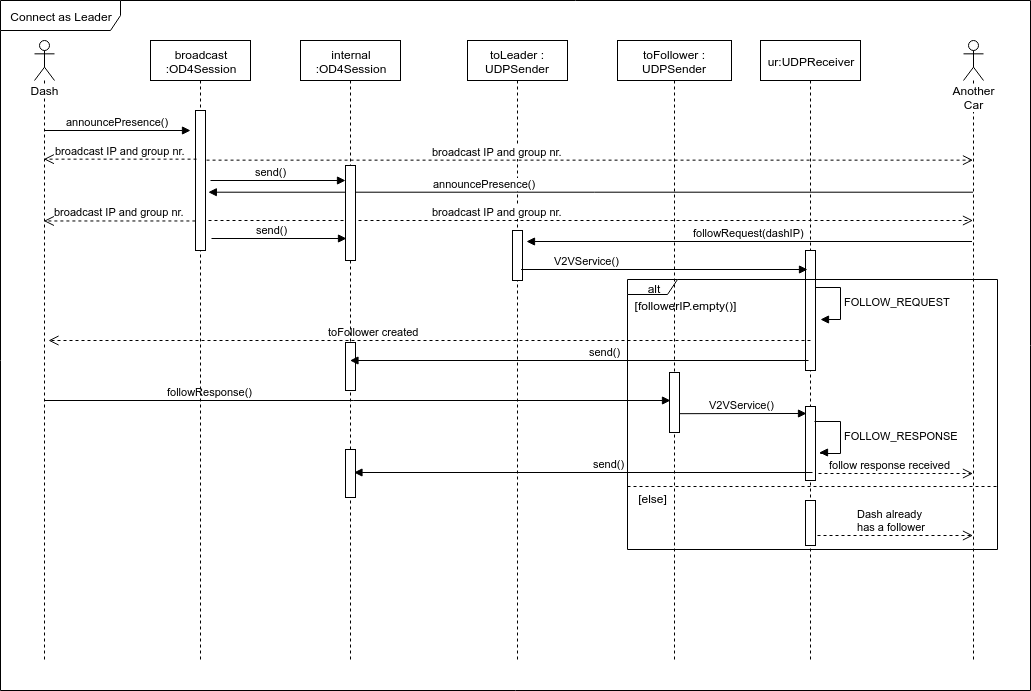
\includegraphics[width=\linewidth]{Diagrams/ConnectAsLeader.png}
\caption{Connect As Leader SD}
\label{fig:stopfollowing}
\end{figure}
\FloatBarrier % -> Wrap image with this, to make sure text does not go infront of image if theres room

\subsubsection{Behaviour}
The interactions begins with both car announcing their presence, to obtain the cars' IPs and IDs. Once this is done Another Car sends a FollowRequest and Dash responds with FollowResponce or ignoners the message in case Dash already has a follower. All messages are forwarded to the internal communication channel as well. The behaviour is identical to the one seen in section \ref{subsubsec: follower bahaviour}. \par

%%%%%%%%%%%%%%%%%%%%%%%%%%%%%%
%%% Stop Following
\subsection{Stop Following}
\subsubsection{Significance}
This use case is the least significant out of the established use cases. It was chosen as it realizes the logic for closing established connection between the cars, a mandatory behaviour from the V2V-Protocol. This is the only use case depicting or incorporating this type of behaviour.  
% Adding image
\FloatBarrier % -> Wrap image with this, to make sure text does not go infront of image if theres room
\begin{figure}[ht!]
\centering
% Make image as wide as the line
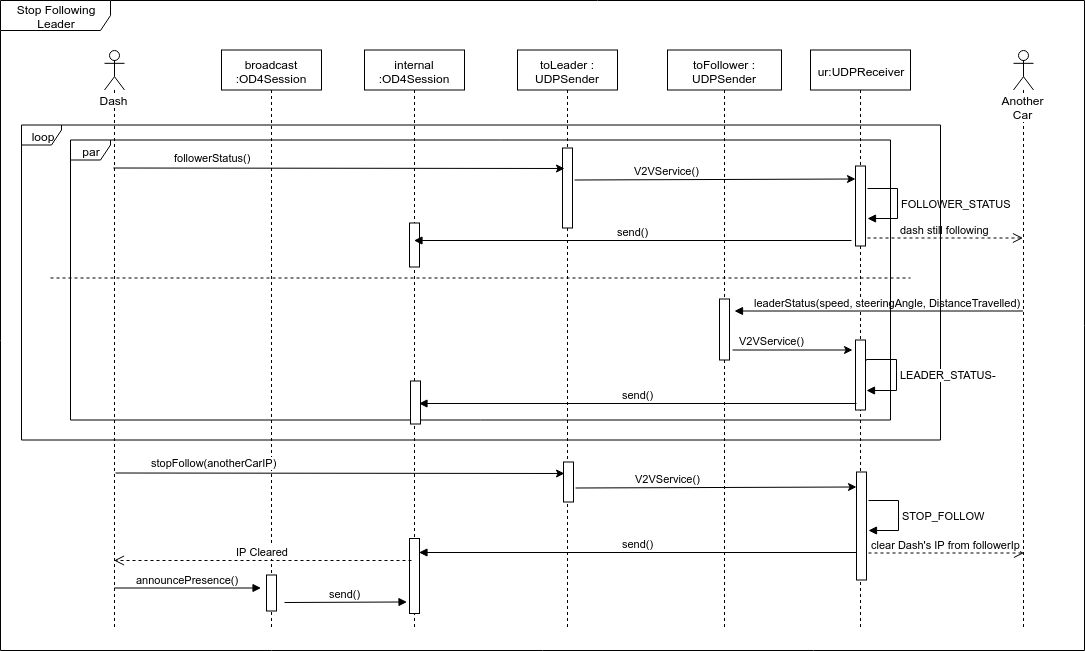
\includegraphics[width=\linewidth]{Diagrams/StopFollowing.png}
\caption{Stop Following SD}
\label{fig:connectasleader}
\end{figure}
\FloatBarrier % -> Wrap image with this, to make sure text does not go infront of image if theres room

\subsubsection{Behaviour}
This use case scenario requires the connections to be established and messages sent. This can be seen via the loop in the sequence diagram. The "par" box is used to depict the messages being sent in parallel. Dash send the StopFollow message to close the UDP connections and wipe the IP. It is important to mention that the exact same behaviour applies regardless of Leader/Follower role.

%%%%%%%%%%%%%%%%%%%%%%%%%%%%%%
%%% New Subsection
\subsection{Maneuvering}

\subsubsection{Importance}
The maneuvering behavior in divided into two parts. The first is driving as a Leader, the second driving as a Follower. The combined action of these two behaviours realize the "Drive Car" user case, see section \ref{us:drive car}. 

\subsubsection{Behaviour}


% Adding image
\FloatBarrier % -> Surround image with this, to make sure text does not wrap
\begin{figure}[ht!]
\centering
% Make image as wide as the line
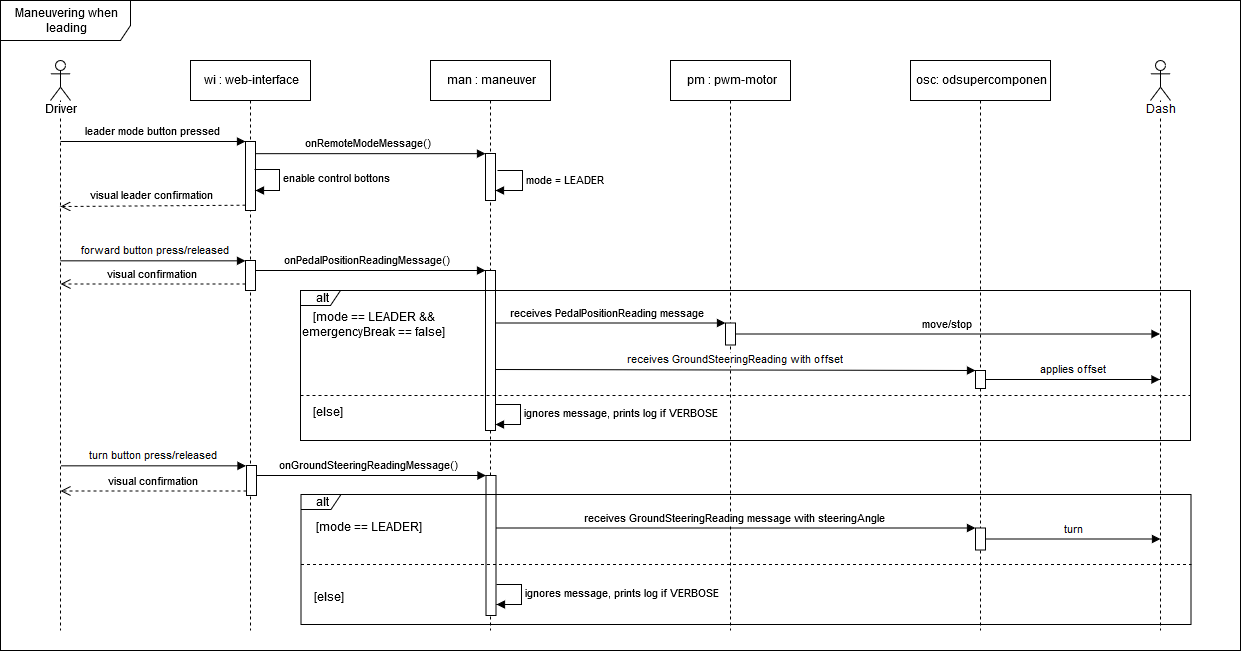
\includegraphics[width=\linewidth]{Diagrams/SequenceDiagramsManeuveringLeader.png}
\caption{Sequence Diagram - Leader}
\label{fig:SD_maneuvering_leader}
\end{figure}

The diagram above depicts the chain of events when controlling the car through the web-interface. Note that turn and forward buttons can be pressed without any particular order. However, leading mode must be enabled for the microservice to evaluate the commands. In case leading mode is enabled and emergencyBreak is false (true in case an obstacle is detected by ultrasonic sensor within a specified distance), commands to move or stop will be forwarded to the pwm-motor microservice. Lastly, commands to turn the servo and thus the car is directly forwarded to the odsupercompontent as long as leading mode is activated. 

\FloatBarrier % -> Surround image with this, to make sure text does not wrap
% Adding image
\FloatBarrier % -> Surround image with this, to make sure text does not wrap
\begin{figure}[ht!]
\centering
% Make image as wide as the line
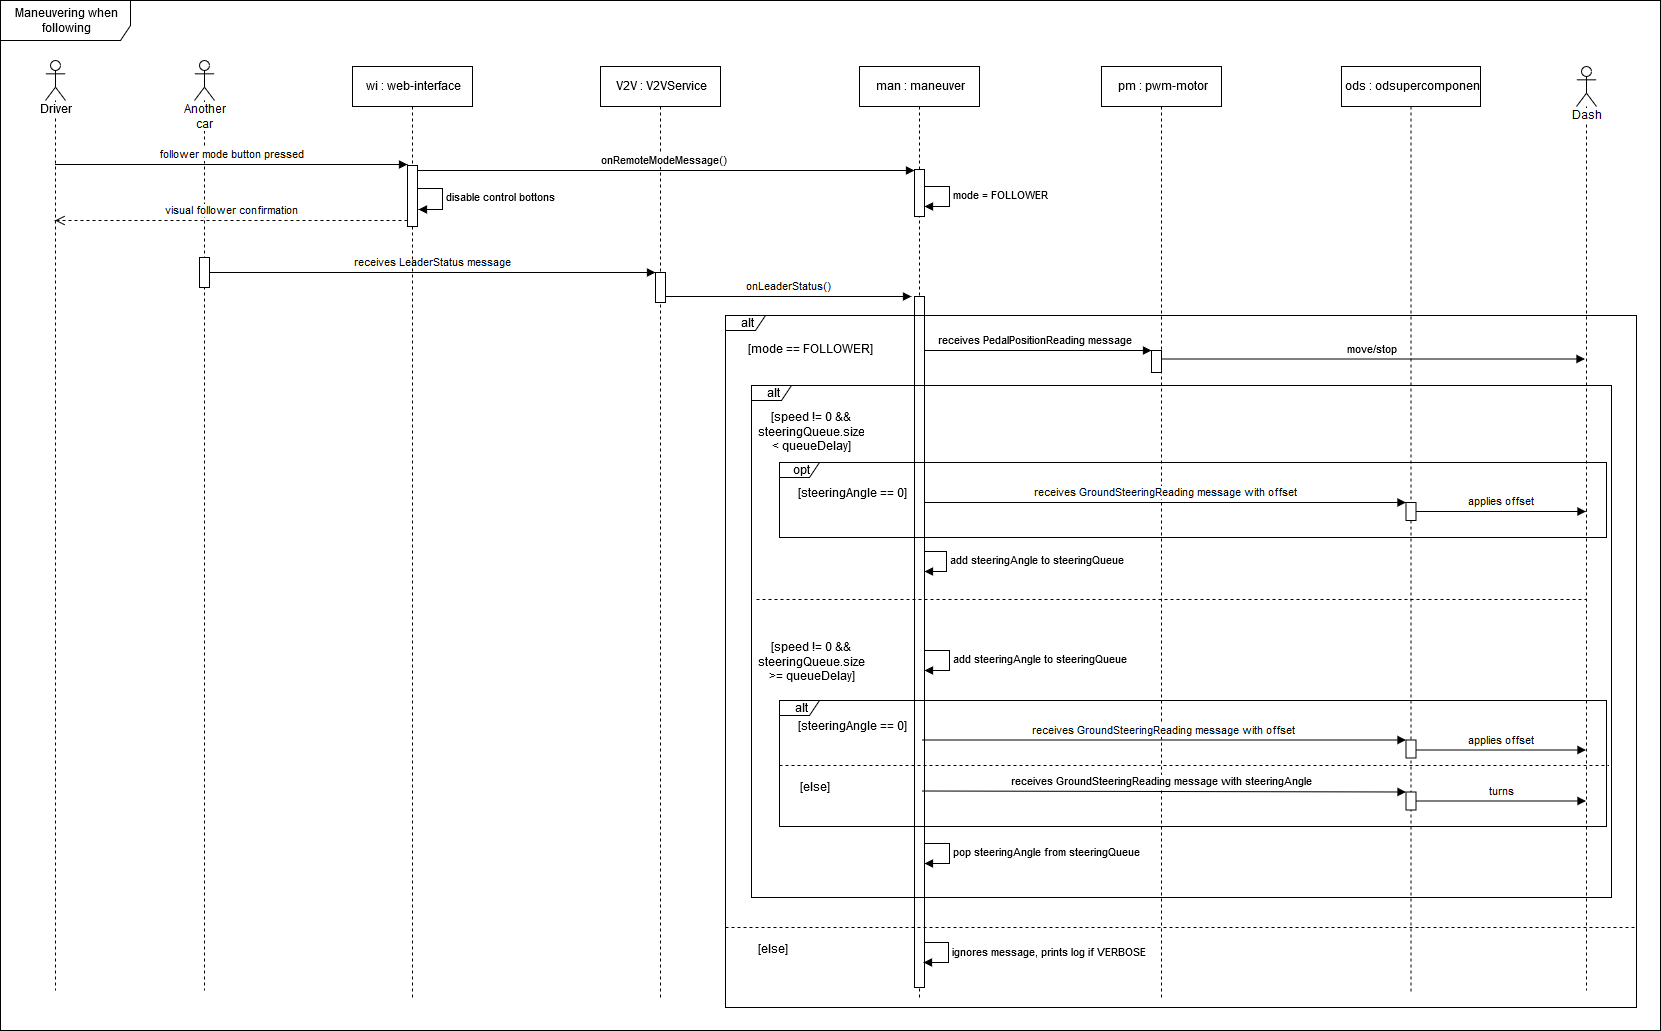
\includegraphics[width=\linewidth]{Diagrams/SequenceDiagramsManeuveringFollower.png}
\caption{Sequence Diagram - Follower}
\label{fig:SD_maneuvering_follower}
\end{figure}
\FloatBarrier % -> Surround image with this, to make sure text does not wrap

Similarly to the first sequence diagram, the diagram above illustrates the chain of events when the car is executing commands. However, instead of having a driver controlling the miniature vehicle directly through the web-interface, the car is following another miniature car autonomously. This is made possible through the retrieval of so called 'LeaderStatus' messages from the leading vehicle. This message is evaluated and processed and eventually a command is sent to the microservices odsupercomponent and pwm-motor for the car to move.


%%%%%%%%%%%%%%%%%%%%%%%%%%%%%%%%%%%%%%%%%%%%%%%%%
% Adding Logical View
%%%%%%%%%%%%%%%%%%%%%%%%%%%%%%%%%%%%%%%%%%%%%%%%%
\section{Logical View}
This section aims to provide a logical overview of the overall structure of the product. The intended audience for this section is someone seeking fundamental understanding of the developed system, and will therefore describe necessary architectural and design decisions on a high level. 

Visualized in Figure \ref{fig:classDiagramLogigal} are the relevant components and their connections in the dashFTABs system. 

'odsupercomponent' and 'pwm-motor' both are components that were provided to the development team by the product owner. The use of microservices are consistent throughout, and was a considered decision made in the inception of the project. For the rationale of this decision, please refer to \ref{microservice rationale}.

The communication line between all components shown here makes use of the Libcluon library, also provided by the project's product owner. The message exchange is done through 'OD4 sessions': utilizing channels and assigning ID's to messages, in this context referenced to as 'CID's. For further explanation of the channels, refer to \ref{microservice rationale}.
% Adding image
\FloatBarrier % -> Wrap image with this, to make sure text does not go infront of image if theres room
\begin{figure}[h]
\centering
% Make image as wide as the line
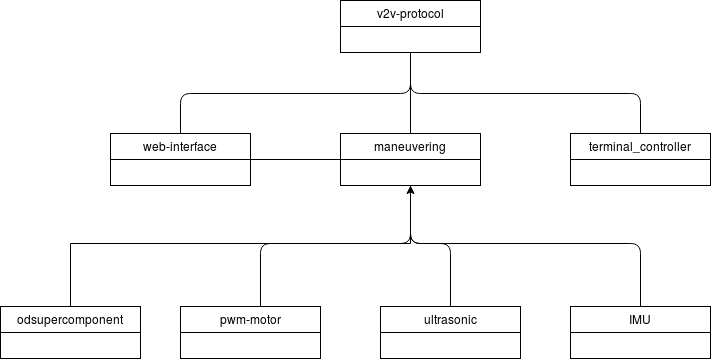
\includegraphics[width=\linewidth]{Diagrams/logical_view.png}
\caption{Simple Class Diagram}
\label{fig:classDiagramLogigal}
\end{figure}
\FloatBarrier % -> Wrap image with this, to make sure text does not go infront of image if theres room

\pagebreak

%%%%%%%%%%%%%%%%%%%%%%%%%%%%%%%%%%%%%%%%%%%%%%%%%
% Adding Physical view
%%%%%%%%%%%%%%%%%%%%%%%%%%%%%%%%%%%%%%%%%%%%%%%%%
\section{Development View}
Deciding on architecture is a vital part of any project, thinking of what benefits a team can reap from the choice during the phases of development. During presentations by Dr. Rev. Christian Berger, it became quite obvious that their architecture of choice was microservices. The team had discussion about the pros and cons of this, see section \ref{microservice rationale}. 

One of the benefits of not choosing the microservice architecture was going for a more familiar architecture that the developers have experience working with. During early discussions, the development team did not find enough reason to not try the new way of designing the system.

% Adding image
\FloatBarrier % -> Surround image with this, to make sure text does not wrap
\begin{figure}[ht!]
\centering
% Make image as wide as the line
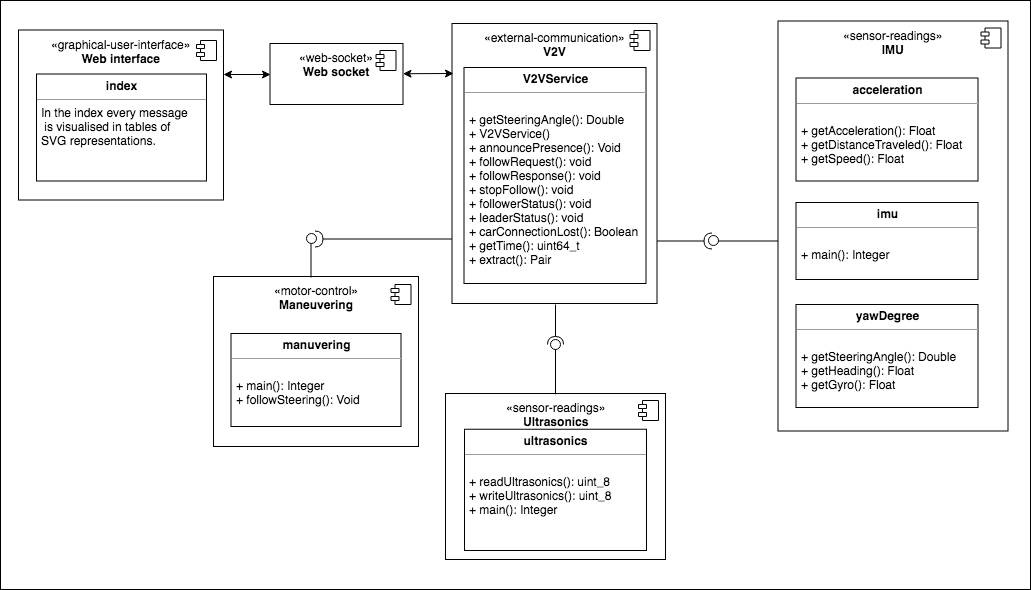
\includegraphics[width=\linewidth]{Diagrams/StructuredClassDiagram.png}
\caption{Structured class diagram}
\label{fig:Structured_class_diagram}
\end{figure}
\FloatBarrier % -> Surround image with this, to make sure text does not wrap

\subsection{V2V Service}
Designed with the V2V Service as a central node in our architecture we can easily route data throughout the system using different CID:s. The project uses multiple connection channels in the V2V Service:
\begin{enumerate}
\item Internal [Channel 122]
This channel is used by the system for internal communication. The internal channel was a design decision based on scalability of our system. Utilizing this channel every part of our system can easily access the data needed to visualize or execute actions accordingly.
\item Broadcasting [Channel 250]
This channel has some of the messages for the external systems in our environment. The external systems are composed out of other groups cars.  The message, at the moment of writing this,  using the channel is the announce presence. If there is a need to send more messages in this channel it can be developed further.
\item Incoming [UDP Connection]
This UPD connection reroutes the incoming messages from other vehicles into the internal channel. When the messages have been distributed, the rest of the system can use the Internal channel OD4 session to access this data. 
\item To Leader [UDP Connection]
This channel is used to send messages to the leader car. This is based on the V2V protocol that all groups use, the protocol gives us a straightforward implementation to exchange data between the cars. 
\item To Follower [UDP Connection]
The follower channel sends status updates to the follower car, the messages sent through this channel gives a uniform understanding of the current position of the cars of interest. 
\end{enumerate}

\subsection{IMU}
To use the IMU on the BeagleBone board some calculations were needed to be conducted. This microservice has the calculations of the returned data from the IMU hardware component.  

The IMU is used to get the change in heading, distance traveled and speed of the car. It broadcasts the data through an enveloped message to the internal channel. 
\subsection{Maneuvering}
The maneuvering microservice is the connection to the actual hardware of the car, it sends the messages from the V2V microservice to control the vehicle. It is designed with two modes, one follower, and one leader. The mode is supposed to decide what messages are interesting to the miniature car.
\subsection{Ultrasonics}
The ultrasonic microservice gives the distance in front of the car, it reads the values from the connected hardware component on the car. The rationale for this service was mainly the emergency brake event. The plan was to use a dynamic user-set distance, which should stop the car instantly. In the future, this could provide redundancy with other components to secure the execution of the emergency brake.
\subsection{Web Interface}
To control the car manually and visualize the internal working of the system, it was decided to use an extension of Chalmers Revere's signal viewer\cite{signal viewer}. In this microservice, we integrated the manual controls as arrow keys and divided the messages into internal and external, to make the visualization a bit clearer. The external messages are everything sent by the V2V Protocol, whereas the internal messages are the data transfered with the project group's vehicle. The IMU and the ultrasonic sensor is represented in animated images, this gives the user a better experience when using the system.  
\subsection{Terminal Controller}
As an interface for testing the car during the project, another microservice, the Terminal Controller, was used. It was developed for simplicity and stability. Initially, the web-interface was a bit lacking in performance and the terminal controller could be used as a backup. Having a backup microservice to use when needed increases the redundancy of the development process, but provides the system users with a backup remote controller that could be used for testing purposes and web-interface validation. 

\subsection {Rational for Microservices} \label{microservice rationale}

Using the aforementioned microservices when working with an embedded system that contains not only our own services, but also microservices created by other developers, gave us a more modifiable system. When microservices are paired with Docker or other operating-system-level virtualization techniques, the whole system becomes fully portable. Moreover, as a whole, a shared vision and knowledge sharing between developers was easier to convey. 

If the team were to continue developing the solution for the autonomous driving or graphical user interface this type of architecture has the power to scale seamlessly as an infinite number of additions can be developed with ease.

One of the bad things with the chosen architecture was, what should each of the services contain, how small should they be and how can we make sure there is no overlap in functionality in the system. In our case, the solution was partly to have a predefined process to ensure that aforementioned shortcomings were mitigated. Even if this process needed to be improved, the practice of dividing the work was carried over from earlier endeavours for the majority of our team. 

When pressed for time, a microservice based architecture can be a large benefit due to the enabling of parallel development of the different services. Anything developed should be able to run independently from everything else in the system. This gave us the ability to test, format and refine each service without having to worry about any other developers work progress. Delivering for each deadline during the project was uncomplicated to monitor, everyone knew who needed to do what part and could help accordingly.
\pagebreak

%%%%%%%%%%%%%%%%%%%%%%%%%%%%%%%%%%%%%%%%%%%%%%%%%
% Adding Physical view
%%%%%%%%%%%%%%%%%%%%%%%%%%%%%%%%%%%%%%%%%%%%%%%%%
\section{Physical View}
A deployment diagram, as seen in Figure \ref{fig:deploymentdiagram}, was created to visualize the distribution of software amongst hardware. The software was deployed onto a BeagleBone. Most of the software developed was encapsulated within Docker images, with few exceptions. \par

The communication between the microservices is done using OD4 Sessions provided by libcluon\cite{libcluon}, as such libcluon is either installed or included as a header only library in each microservice. Moreover, each microservice includes, at the minimum, a Messages.odvd file that defines message specification and an OD4 Session to transfer the readings to an internally defined OD4 channel, expressed with CID 122. \par

The "ultrasonic" and "imu" microservices were built as executables as the dependent libary \cite{robotics cape} was not able to be encapsulated within docker images.

% Adding image
\FloatBarrier % -> Surround image with this, to make sure text does not wrap
\begin{figure}[ht!]
\centering
% Make image as wide as the line
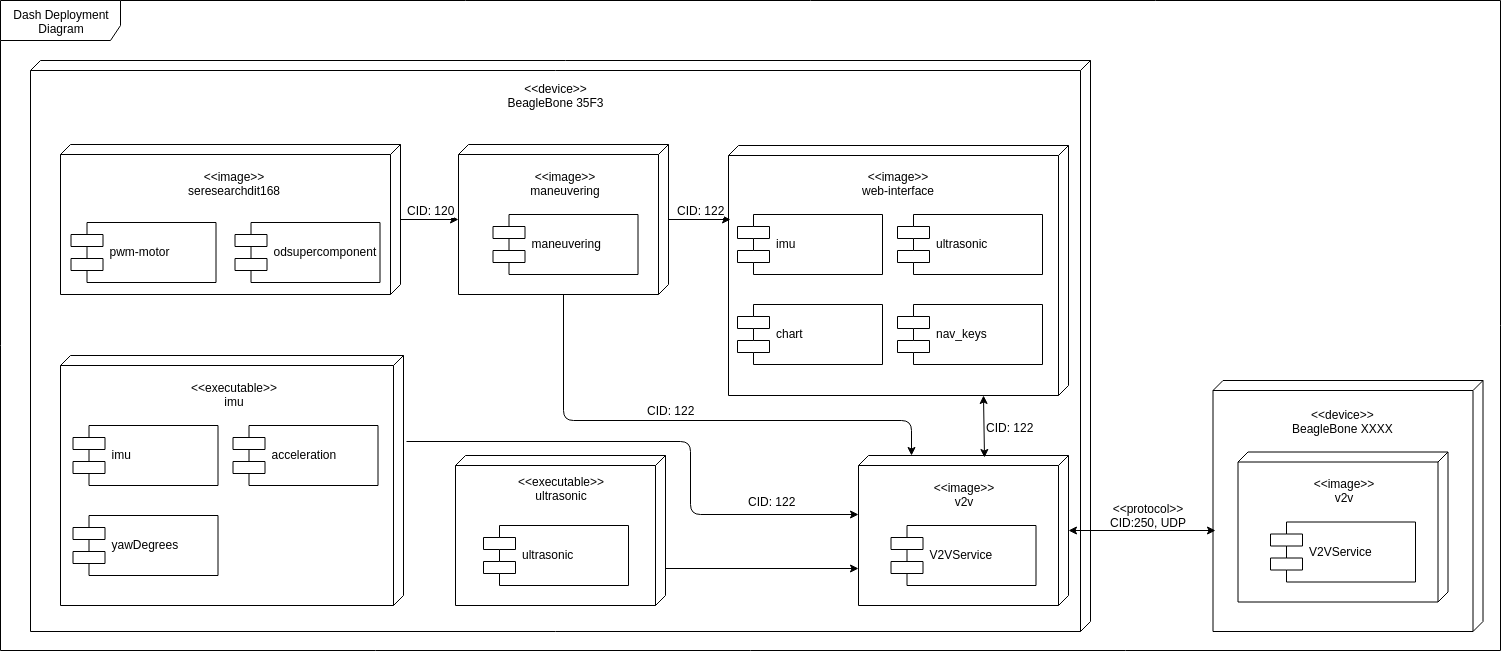
\includegraphics[width=\linewidth]{Diagrams/DeploymentDiagram.png}
\caption{Deployment Diagram}
\label{fig:deploymentdiagram}
\end{figure}
\FloatBarrier % -> Surround image with this, to make sure text does not wrap

\pagebreak

%%%%%%%%%%%%%%%%%%%%%%%%%%%%%%%%%%%%%%%%%%%%%%%%%
% Adding Bibliography
%%%%%%%%%%%%%%%%%%%%%%%%%%%%%%%%%%%%%%%%%%%%%%%%%
\begin{thebibliography}{9}
	\bibitem{FinalReport} Laurin, E., Törnqvist, I., Eberlen, J., \& Stirbys, J. Final Report, GitHub repository:
\url{https://github.com/justasAtGU/dit168/tree/master/doc/ProjectManagement/FinalReport}
	\bibitem{libcluon} Berger, C., libcluon, GitHub repository: \url{https://github.com/chrberger/libcluon}
	\bibitem{ultrasonics} Chalmers Revere, GitHub repository; \url{https://github.com/chalmers-revere/opendlv-device-ultrasonic-srf08}
    \bibitem{robotics cape} Strawson Design, Robotics Cape, Website: \url{http://www.strawsondesign.com/\#!}
	\bibitem{signal viewer} Chalmers Revere, GitHub repository: \url{https://github.com/chalmers-revere/opendlv-signal-viewer}
\end{thebibliography}
\end{document}
